
\chapter{Methodology}

The current technical report involves an explanation of the HRI connection,
the HRI application, and the hand gesture control algorithm.
% , and a briefly information of the wireless accelerometer trans-receiver and the patrol mobile robot.

\section{HRI Setup}

In order to use the HRI application, a scheme setup is shown in  Figure~\ref{fig:hbd}, and the
following steps are provided as an explanation of HRI connection:
% \begin{figure}[tbp]
\begin{figure}[h!]
  \begin{center}
  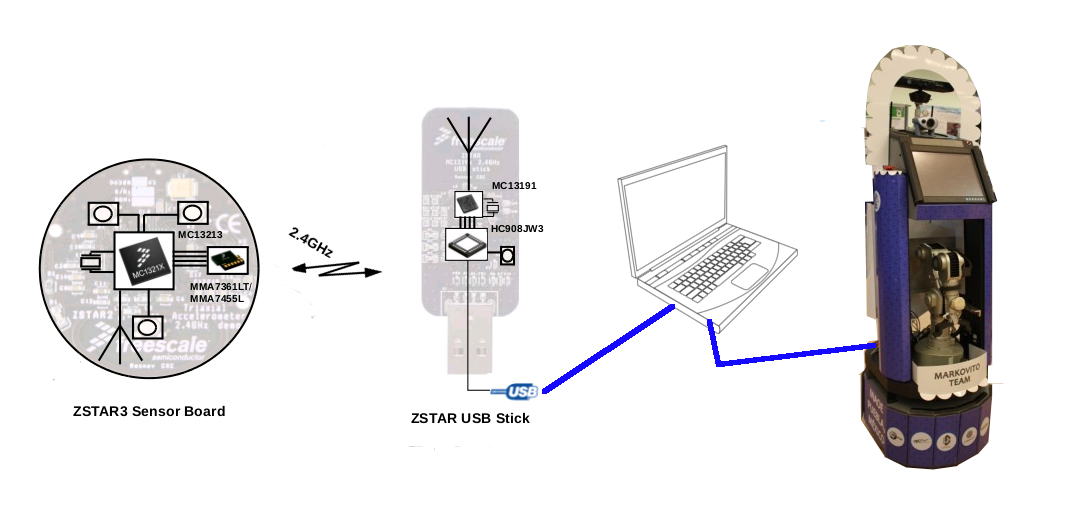
\includegraphics[scale=.3]{hridd-blockdiagram}
    \caption[HRI]{Human-Robot Interface Dance Demo Scheme Connection}
    \label{fig:hbd}
  \end{center}
\end{figure}


\begin{enumerate}
 \item Turn on the Pioneer Mobile Robot
 \item Connect the Aria USB Connector and the ZSTAR USB Stick to the available laptop's USB plugs.
 \item The user must strictly wear  the USB sensor board on his/her left wrist  as shown in Figure~\ref{fig:wsb}, 
 and it is important to emphasize that similar sensor position is crucial to obtain same results.
 \item Finally, turn on the sensor board by pushing any of the three white pushbuttons.
\end{enumerate}


% \begin{figure}[tbp]
\begin{figure}[h!]
  \begin{center}
  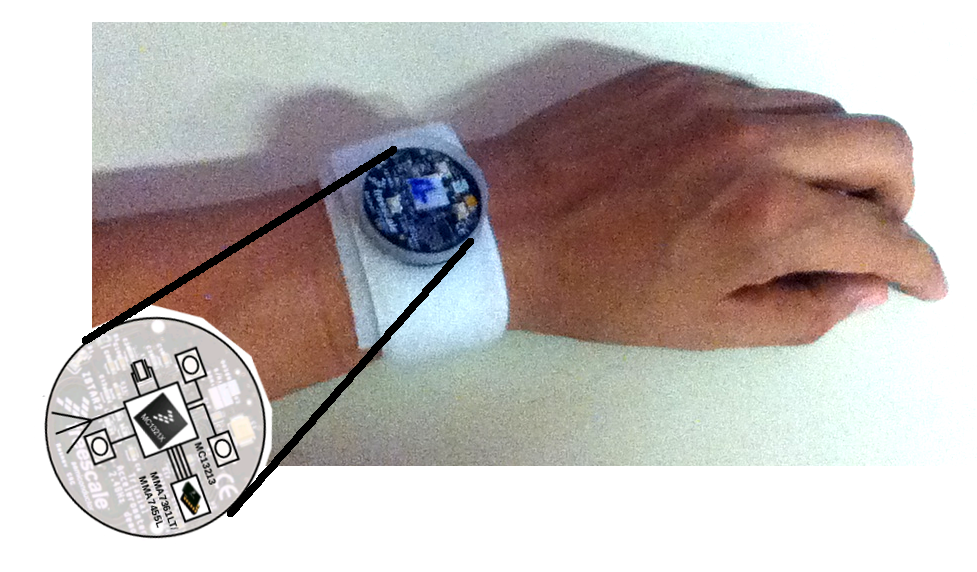
\includegraphics[scale=.3]{wsb}
    \caption[HRI]{Wearable Sensor Board.}
    \label{fig:wsb}
  \end{center}
\end{figure}



For more detailed information about the Wireless Sensing Triple Axis Reference (ZSTAR3) 
and the patrol mobile robot, please visit the references \cite{zstar, probot}.



\section{HRI Application}

You should first download the source tarball from 
\href{https://sites.google.com/site/perezxochicale/projects/demodance/cpp-source-code/hridancedemo-0.0.1.tar.gz}{hridancedemo-0.0.1.tar.gz}
, then uncompress it using: \verb|$tar xzvfp hridancedemo-0.0.1.tar.gz|.

After uncompressing, a new directory in \verb|~/(hridancedemo-0.0.1)| will have been
created. Go into \verb| ~/dancedemoapp/|directory and 
change the executable permissions and finally run the application by using the following commands lines:\\

\verb| $ cd ~/dancedemoapp/|  \\

\verb| $ sudo chmod +x usbresetapp dancedemoapp|  \\

\verb| $ sudo ./dancedemoapp|

Once the application is running, the accelermoter data is displayed at the terminal,
and whenever you want to stop the application you should hit any key.

\section{Hand Gesture Recognition Algorithm}
While running the application, the user is able to move his/her hand in four different gestures in order to move the robot
as is illustrated below in Figure~\ref{fig:pfs}.
% \begin{figure}[tbp]
\begin{figure}[h!]
  \begin{center}
  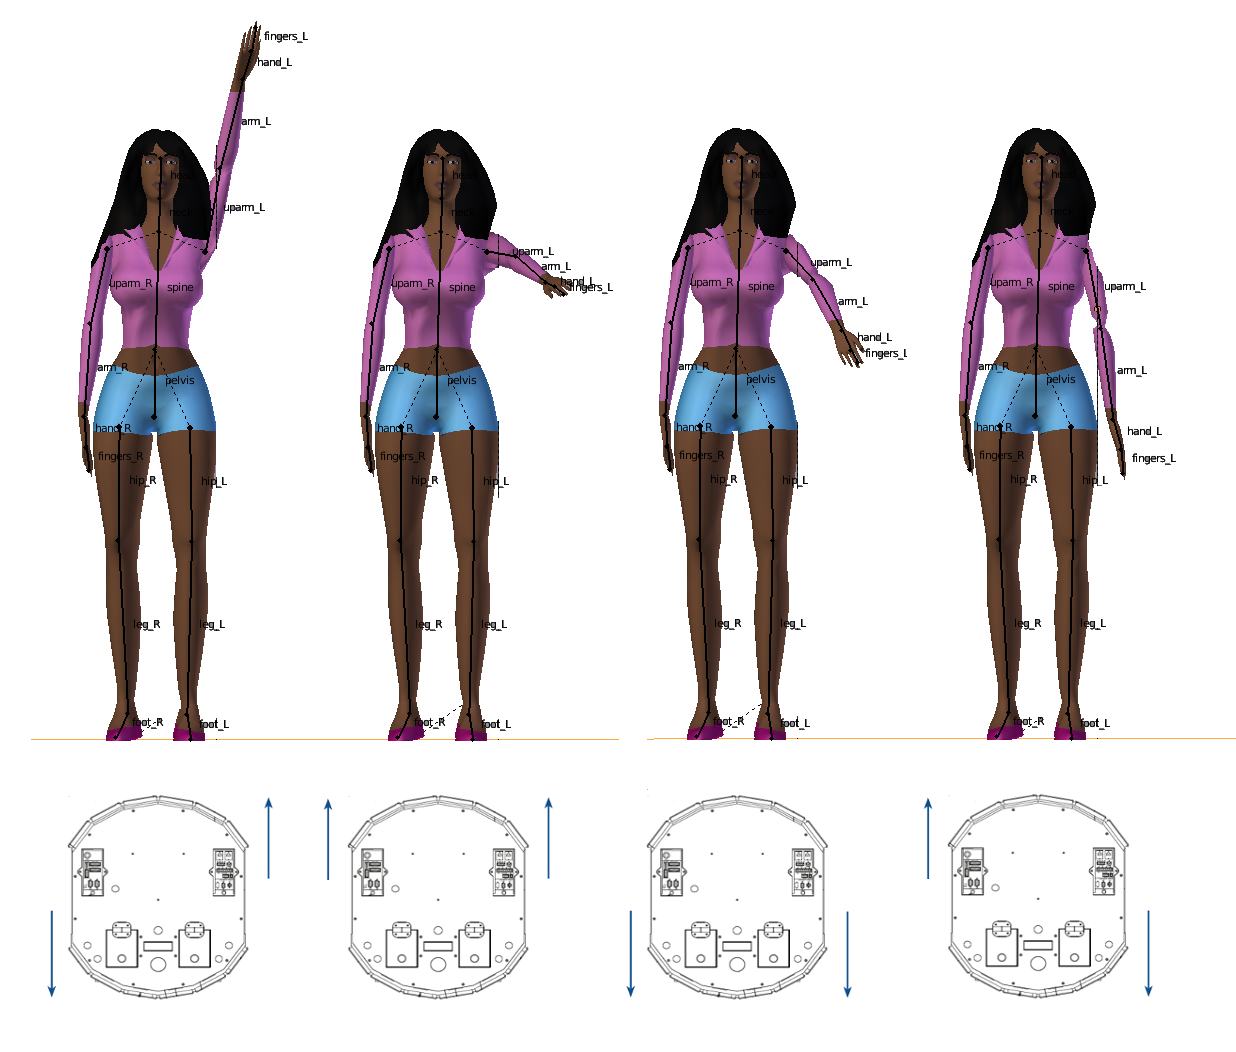
\includegraphics[scale=.28]{demodance}
%     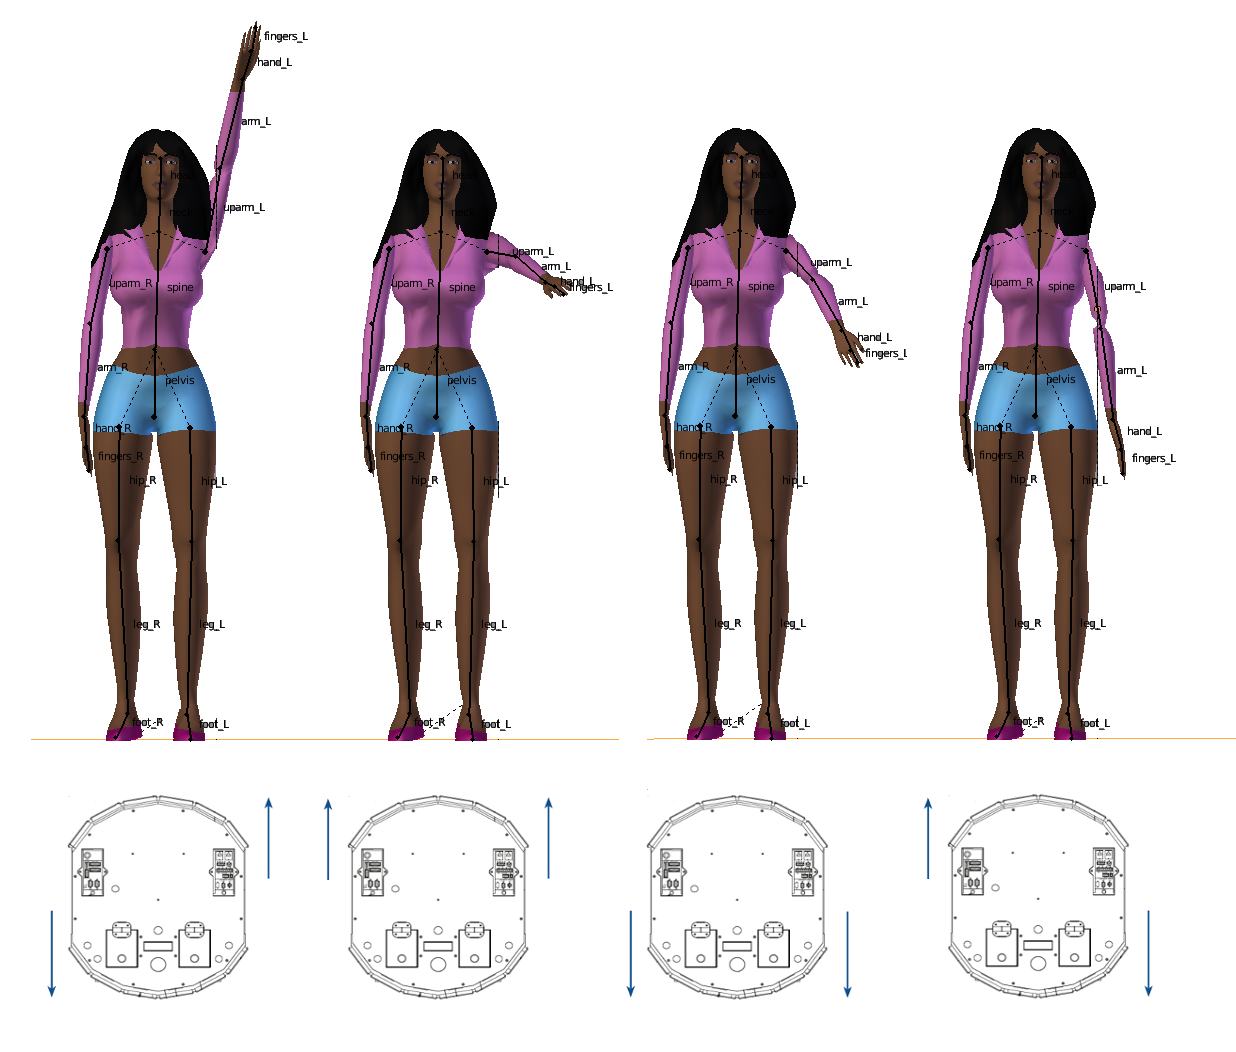
\includegraphics[width=0.7\textwidth]{demodance}
%     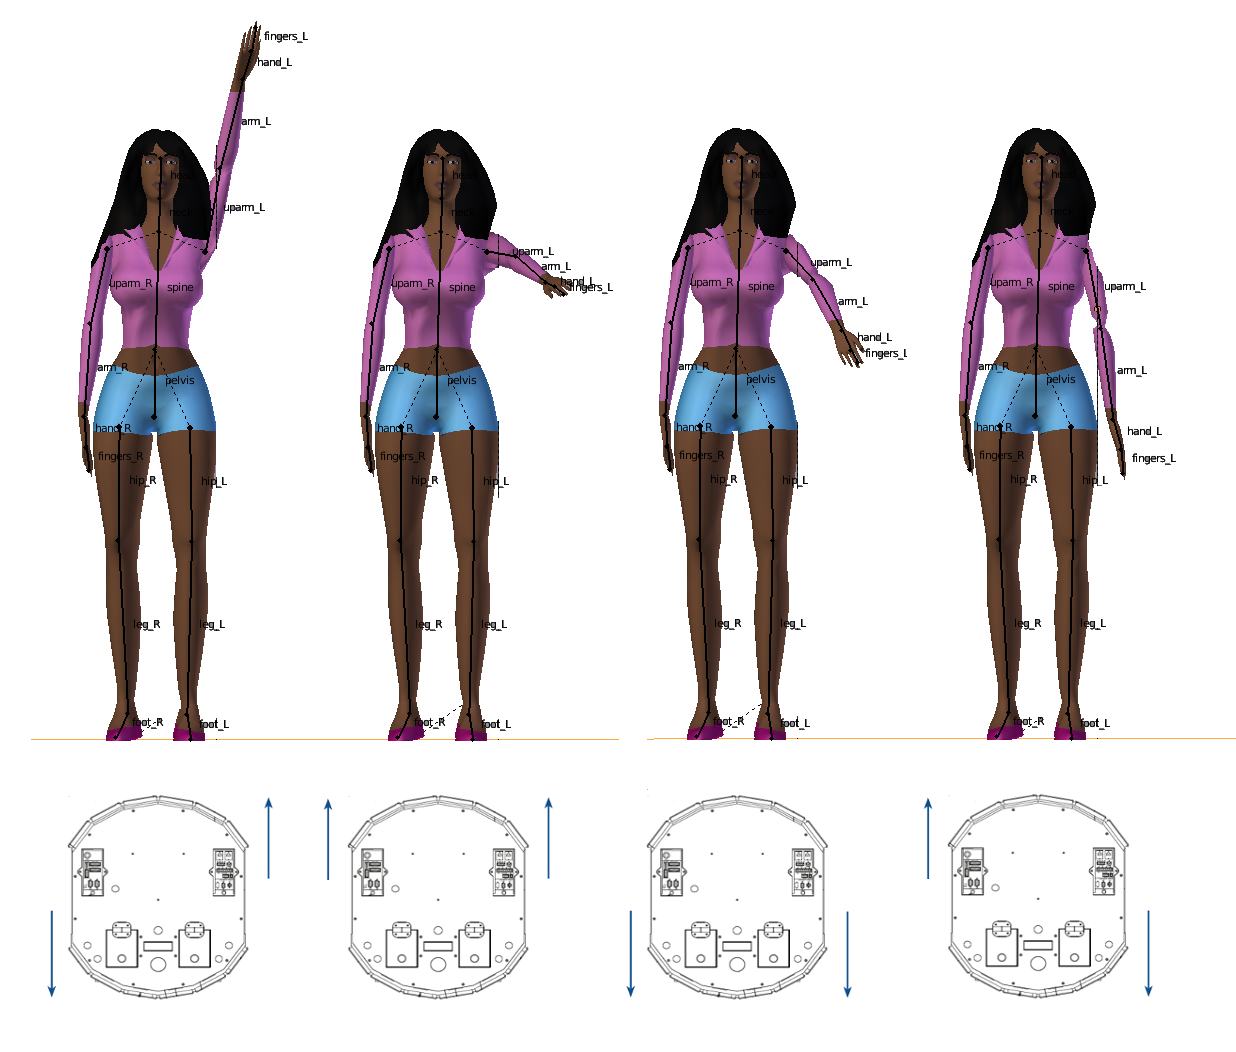
\includegraphics{demodance}
    \caption{User's Left Hand Gestures with the robot's movements arrow directions.}
    \label{fig:pfs}
  \end{center}
\end{figure}


% Reading an real-time of the data accelerometer is quite important. 
Hence, having read the $X, Y, Z$ accelerations from the sensor board, the arithmetic mean and the variance 
is computed by using the Equations \ref{eq:msd}.
\begin{eqnarray}
 \mu =\frac{1}{n}\cdot \sum_{i=1}^n{x_i},  \quad \operatorname{Var}(X)= \frac{1}{n} \sum_{i=1}^n (x_i - \mu)^2. 
             \label{eq:msd}
\end{eqnarray}

 During the demo, the acceleration data of the accelerometer is collected and
represented as a frame of 5 samples in order to obtain the mean and standard deviation.
As a result of that, a control algorithm was implemented and it is described in (\ref{code:hridd}). 
The complete C++ source code is abailable in the Appendix A.


% The four gestures  described on (algorithm (\ref{code:hridd}))
% % The arithmetic mean is the "standard" average, often simply called the "mean".
% an algorithm is implemented with the 
% we develop an algorithm (\ref{code:hridd})
% for four gestures.


\begin{algorithm}[h!]
  \caption{An example for format For \& While Loop in Algorithm}
  \begin{algorithmic}[1]
%   \State $i=1$
%   \State $FRAMEINTERVAL=5$
    \While {!kbhit()}  
      \State Accelerometer Adquisition Data 
%       \State ACCacumulator
            \If { (iteration mod FRAMEINTERVAL) $== 0$ }
		\State  compute the mean and standard deviation
		\If { $(\mu_X < 1.1)$  and $\mu_X > 0.5$ } 
		\State Robot Spin to the left at 150 mm per second
		\EndIf
		
		\If { $\mu_X < 0.5$  and  $\mu_X > -0.3$ }  
		    \If {$\mu_Y > 0.5$}
		    \State Robot move fordward at 120 mm per second
		    \Else 
		    \State Robot move backward at 120 mm per second
		    \EndIf
		\EndIf
		
		\If { $\mu_X < -0.3$  and  $\mu_X > -1.1$ } 
		\State Robot Spin to the right at 150 mm per second
		\EndIf		
	
% 	   \State  Clearing ACCacumulator
	   \EndIf
	   
	   
%     \State increment i
  \EndWhile
  \label{code:hridd}
  \end{algorithmic}
\end{algorithm}



